\section{Results\label{sec:results}}
  
  Benchmarking of a \gls{usp} implementation before and after the optimisations presented in the previous section have been applied, were collected using both a static diagnostic model and one representative of a physical particle simulation. All data presented was collected using an NVIDIA Titan-X (Pascal) in TCC mode with CUDA 8.0 on Windows 10.
  
  In each benchmark the model is executed for 500 iterations. During each iteration the overall execution time in addition to separate timings for both the message emission and neighbourhood search stages are collected. However for the purposes of this research, the optimisations do not affect the construction of the \gls{usp} data structure, only the neighbourhood search timings are presented within this section.
  \note{Could submit full data sets as a digital-only appendix}
  
  \subsection{Static Uniform Access}
    Under the diagnostic model, each thread is allocated a location. The location is both emitted as a message and used as the central point for a \gls{frnns} search. During the search the neighbour locations are averaged, this ensures both that optimisation has not removed necessary elements of the search and that we have a suitable export for validation between builds.
  
    Two modes of initialisation have been used: uniform and uniform random. The uniform initialisation positions messages so that they are in an equally distributed grid. Whilst uniform ensures agents are strictly uniformly distributed through the environment, when the spacing of the environment is not a factor of the neighbourhood radius this can lead to uneven populations between bins. The uniform random initialisation utilises the CUDA device function \lstinline{float curand_uniform(curandState_t *)} to position messages within the environmental bounds, essentially producing a noiser version of the uniform initialisation. To ensure consistency when using random initialisation, the same seed value was used to initialise comparative benchmarks between builds.
    \note{Could detail the uniform init algorithm}
    
    The diagnostic model has been carried out in both two and three dimensions, across a two dimensional parameter space collecting results from a total of 75,000 parameter combinations. Agent populations from 10,000 to 300,000 have been tested with average neighbourhood volumes from 17 to 430.
    \subsubsection{2D}
      
      \textit{A little stumped on the best way to present the results. We have 2D parameter sweeps in two and three dimensions, with uniform and uniform random initialisation. The 2D parameter sweep of two dimensions has a total of 300k data points, I can produce a cross-sectional graph of this data at any point. Whilst there is a slight difference between uniform and uniform random, that is most often presented via uniform having noisier data (for reasons explained above). Of the 75k configurations executed, less than 1\% were lost by hybrid, and those loses were essentially equal perf as opposed to a loss. Although graphs at the necessary scale to fit a column in the paper will be very unclear in greyscale. See Below}

\begin{figure}[!t]
\centering
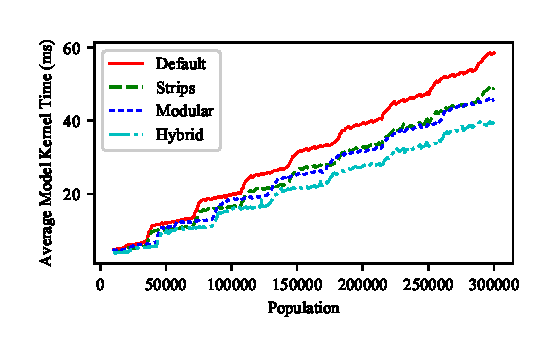
\includegraphics[width=\linewidth]{../resources/results/sample.eps}
\caption{\label{fig:sample-graph}A sample of the kind of graph I'm expecting to produce.}
\end{figure}
    \subsubsection{3D}

  \subsection{Physical model}
    The physical model used is an extension of that proposed by Chisholm et al as a means for benchmarking \gls{frnns} using a simple particle model analogue.\cite{CRM16} The extension modifies the force calculation to utilise sin as a means of smoothing. The addition of smoothing reduces the applied forces about the equilibrium position, such that the particle jitter about equilibrium position from the initial model is eliminated. Adittionally this has made it possible to merge the attraction and repulsion parameters.
    
    The new force calculation formula therefore takes the form $F_{ij} = sin(-2\pi(\frac{d_{ij}}{r}))F$, whereby: $d_{ij}$ is the scalar distance between source particle $i$ and neighbour particle $j$, $r$ is the interaction radius and $F$ is the unified force dampening argument. $F_{ij}$ is subsequently multiplied by the normalised direction vector from $i$ to $j$. As with the original model, $F_{ij}$ is calculated for all neighbour particles with the sum of the resulting value providing the final offset that is applied to the source particle.
    
    \textit{Currently running a reduced definition 2D parameter over this model with a fixed force modifier that produces visually appealing results.}
    
    \textit{Brief explanation specific to results}

  \subsection{Concluding analysis (of results)}
    \textit{Wider analysis of results citing profiled analysis to explain limitations of this innovation (careful to not repeat concluding [next] section too much)}

